%% Included in decks: slidemage-manual
%%

% SlideMage manual, chapter "Working in SlideMage": the three options under the
% deck table, and the buttons for other outputs. The crop is the appendix page
% of this manual (tools/manual/make_crops.py). What the checkboxes produce:
% slide 1kg.
\begin{standardframe}{Options and other formats}
	\small
	Besides the checkboxes in each row, the main screen has three options under
	the deck table that change how PDFs are made, and buttons for other outputs.
	\par\smallskip
	\begin{columns}[T,onlytextwidth]
		\begin{column}{0.63\linewidth}
			\textbf{Under the deck table}
			\shrinklists{2}
			\begin{itemize}
				\item \emph{Include footer timestamp}: puts the compile date and time in the footer (off by default)
				\item \emph{Generate appendix TOC}: appends an agenda and clickable slide previews to every whole-deck PDF (also a deck setting)
				\item \emph{Auto-open generated PDFs}: opens each PDF when it is finished
			\end{itemize}
			\textbf{Other outputs}
			\shrinklists{2}
			\begin{itemize}
				\item \emph{Export PPTX} (in the row): a PowerPoint file for recording a lecture, reveal steps fading out one by one
				\item \emph{Create Transcript} (under the table): the accessible text version of a deck
			\end{itemize}
		\end{column}
		\begin{column}{0.34\linewidth}
			\centering
			{\setlength{\fboxsep}{0pt}\fcolorbox{c_primary_gray}{white}{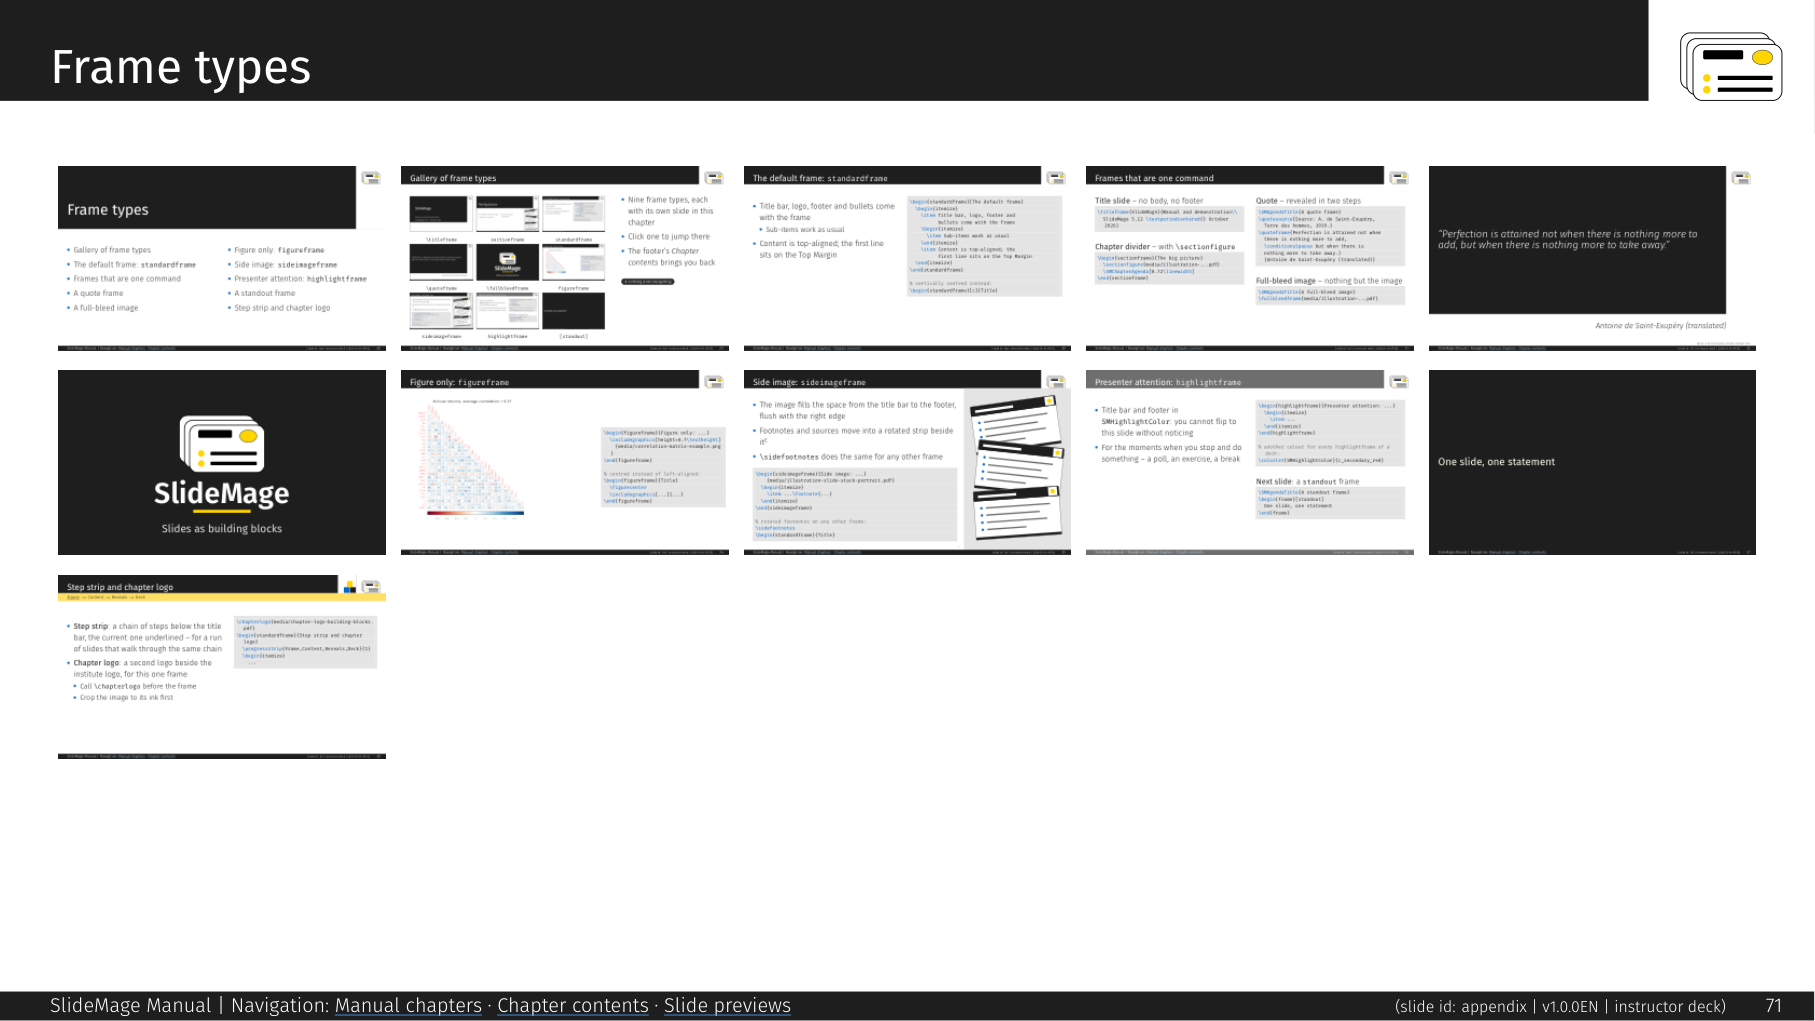
\includegraphics[width=\dimexpr\linewidth-0.8pt\relax]{media/screenshot-slide-appendix-grid.png}}}\par
			{\scriptsize the appendix: a grid of slide previews\par}
		\end{column}
	\end{columns}
\end{standardframe}
